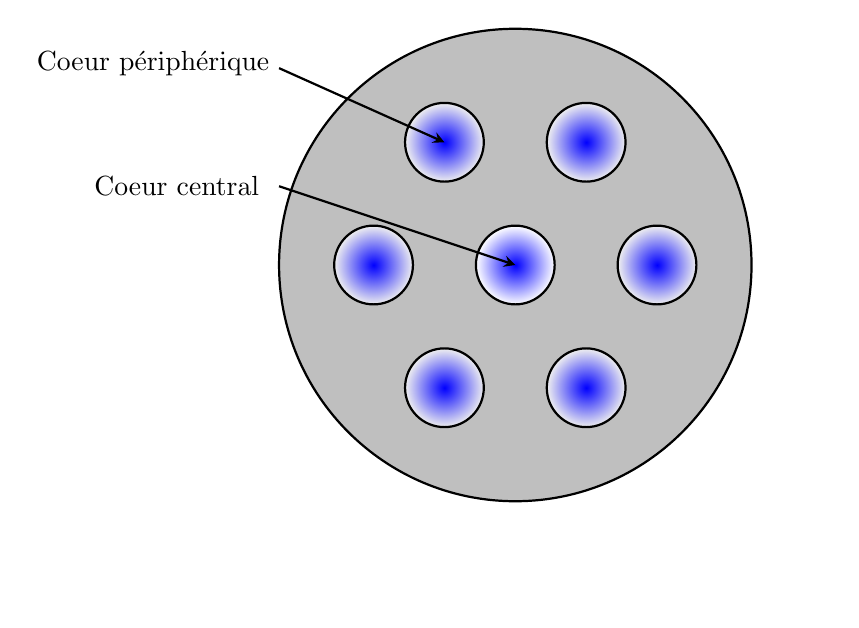
\begin{tikzpicture}[>=stealth]

  %%%%%%%%%%%%%%%%%%%%%%%%%%%%%%%%%%%%%%%%%%%%%%%%%%%%%%%
  % 1) Gaine (cladding) - grand cercle
  %%%%%%%%%%%%%%%%%%%%%%%%%%%%%%%%%%%%%%%%%%%%%%%%%%%%%%%
  \draw[fill=lightgray, draw=black, thick] (0,0) circle (3);

  %%%%%%%%%%%%%%%%%%%%%%%%%%%%%%%%%%%%%%%%%%%%%%%%%%%%%%%
  % 2) Disposition des coeurs
  %    Exemple : 7 coeurs (1 au centre, 6 autour)
  %%%%%%%%%%%%%%%%%%%%%%%%%%%%%%%%%%%%%%%%%%%%%%%%%%%%%%%
  % Rayon du coeur
  \def\rcoeur{0.5}
  % Rayon du cercle imaginaire sur lequel on place les 6 coeurs périphériques
  \def\R{1.8}

  % -- a) Coeur central
  \begin{scope}
    % Pour remplir avec un dégradé (mode fondamental ~ gaussienne)
    \clip (0,0) circle (\rcoeur);
    \shade[inner color=blue, outer color=white]
      (0,0) circle (\rcoeur);
  \end{scope}
  \draw[thick] (0,0) circle (\rcoeur);
  % On stocke la coordonnée du centre pour faire pointer une flèche
  \coordinate (CenterCore) at (0,0);

  % -- b) Les 6 coeurs autour
  \foreach \k in {0,...,5}{
    % Angle en degrés (espacés de 60°)
    \pgfmathsetmacro{\angle}{60 * \k}
    % Coordonnées polaires -> cartésiennes
    \coordinate (C\k) at ({\R*cos(\angle)}, {\R*sin(\angle)});
    
    % On dessine le disque du coeur
    \begin{scope}
      \clip (C\k) circle (\rcoeur);
      \shade[inner color=blue, outer color=lightgray!25!white]
        (C\k) circle (\rcoeur);
    \end{scope}
    \draw[thick] (C\k) circle (\rcoeur);
  }

  %%%%%%%%%%%%%%%%%%%%%%%%%%%%%%%%%%%%%%%%%%%%%%%%%%%%%%%
  % 3) ANNOTATIONS (flèches droites et étiquettes)
  %%%%%%%%%%%%%%%%%%%%%%%%%%%%%%%%%%%%%%%%%%%%%%%%%%%%%%%

  % (a) Flèche vers le coeur central
  \draw[->, thick]
    (-3,1) -- (CenterCore)
    node[xshift = -4.3cm, yshift = 1cm]
    {Coeur central};

  % (b) Flèche vers l'un des coeurs périphériques
  %     Ex: \k=2 (angle=120°) => coeur du haut-gauche
  \draw[->, thick]
    (-3,2.5) -- (C2)
    node[xshift = -3.7cm, yshift = 1cm]
    {Coeur périphérique};

    \draw[white, opacity = 0] (-4,-4.25)  rectangle (4,0);
\end{tikzpicture}


